\section{Технический проект}
\subsection{Общая характеристика организации решения задачи}

Необходимо спроектировать и разработать приложение, который должен способствовать популяризации игр-платформеров.

Приложение представляет собой набор взаимосвязанных различных окон, которые сгруппированы по разделам, содержащие текстовую, графическую информацию. Приложение располагается на компьютере. При разработке используется библиотека Pygame.

\subsection{Обоснование выбора технологии проектирования}

На сегодняшний день информационный рынок, поставляющий программные решения в выбранной сфере, предлагает множество продуктов, позволяющих достигнуть поставленной цели – разработки игрового приложения.

\subsubsection{Описание используемых технологий и языков программирования}

В процессе разработки приложения используются программные средства и языки программирования. Каждое программное средство и каждый язык программирования применяется для круга задач, при решении которых они необходимы.

\subsubsection{Язык программирования Python}

Python –  высокоуровневый язык программирования общего назначения с динамической строгой типизацией и автоматическим управлением памятью, ориентированный на повышение производительности разработчика, читаемости кода и его качества, а также на обеспечение переносимости написанных на нём программ. Язык является полностью объектно-ориентированным в том плане, что всё является объектами. Необычной особенностью языка является выделение блоков кода отступами. Синтаксис ядра языка минималистичен, за счёт чего на практике редко возникает необходимость обращаться к документации. Сам же язык известен как интерпретируемый и используется в том числе для написания скриптов. Недостатками языка являются зачастую более низкая скорость работы и более высокое потребление памяти написанных на нём программ по сравнению с аналогичным кодом, написанным на компилируемых языках, таких как C или C++.

\paragraph{Достоинства языка Python}
\begin{itemize}
	\item Простота и читаемость кода: Python использует простой и чистый синтаксис, что делает код легким для понимания и обслуживания.
	\item Многофункциональность: Python подходит для создания различных типов приложений, включая веб-приложения, настольные приложения, научные вычисления, обработку данных и многое другое
	\item Большой выбор библиотек: Python имеет огромное сообщество разработчиков, что приводит к большому количеству библиотек и модулей для различных задач. Например, для машинного обучения есть библиотека TensorFlow, для веб-разработки - Django, для анализа данных - Pandas и многое другое.
	\item Кроссплатформенность: Python работает на различных операционных системах, таких как Windows, macOS, Linux и другие.
	\item Быстрая разработка: Python позволяет быстро создавать прототипы и тестировать идеи благодаря своей простоте и мощности.
\end{itemize}



\subsubsection{Использование библиотеки Pygame}

\paragraph{Введение}
Библиотека Pygame — это набор модулей Python, предназначенных для создания видеоигр. Она включает в себя компьютерную графику и звуковые библиотеки, разработанные для использования с языком программирования Python. Pygame основана на библиотеке SDL и позволяет разработчикам быстро создавать игры и мультимедийные приложения.

\paragraph{Возможности Pygame}
Вот некоторые из основных возможностей, предоставляемых библиотекой Pygame:

\begin{enumerate}
		\item предоставляет функции для работы с изображениями и анимацией. Разработчики могут загружать, отображать и манипулировать изображениями в различных форматах;
		\item можно воспроизводить звуковые файлы и музыку, а также работать со звуковыми эффектами;
		\item обрабатка ввод данных от клавиатуры, мыши и других устройств ввода, а также управление системой событий;
		\item в библиотеке есть инструменты для работы с векторной графикой и физическими расчетами, что полезно для создания более сложных игровых механик.
\end{enumerate}

\paragraph{Применение библиотеки Pygame в программе}
Модуль game подключает библиотеку pygame. Класс Game внутри модуля game использует библиотеку для инициализации и отображения окна игры, для работы с объектами, для получения состояния всех кнопок клавиатуры, использования графических элементов.
Инициализация библиотеки Pygame.
Пример представлен на рисунке \ref{init:image}:
\begin{figure}[H]
	\begin{lstlisting}[language=Python]
		pygame.init()
	\end{lstlisting}  
	\caption{Инициализация библиотеки pygame в программу}
	\label{init:image}
\end{figure}
Отображение окна игры(используются параметры ширины и высоты).
Пример представлен на рисунке \ref{displaysm:image}:
\begin{figure}[H]
	\begin{lstlisting}[language=Python]
		self.display_surface = pygame.display.set_mode((width, height))
	\end{lstlisting}  
	\caption{Создание окна игры}
	\label{displaysm:image}
\end{figure}
Создание объекта помогающего отслеживать время.
Пример представлен на рисунке \ref{clock:image}:
\begin{figure}[H]
	\begin{lstlisting}[language=Python]
		self.clock = pygame.time.Clock()
	\end{lstlisting}  
	\caption{Создание таймера}
	\label{clock:image}
\end{figure}
Установка заголовка текущего окна.
Пример представлен на рисунке \ref{caption:image}:
\begin{figure}[H]
	\begin{lstlisting}[language=Python]
		pygame.display.set_caption(caption)
	\end{lstlisting}  
	\caption{Установка заголовка}
	\label{caption:image}
\end{figure}
Получение состояния всех кнопок клавиатуры.Возвращает True если была нажата клавиша key, иначе False(например self.key\_pressed(pygame.K\_SPACE)).
Пример представлен на рисунке \ref{keyp:image}:
\begin{figure}[H]
	\begin{lstlisting}[language=Python]
		return pygame.key.get_pressed()[key]
	\end{lstlisting}  
	\caption{Получение состояния всех кнопок клавиатуры}
	\label{keyp:image}
\end{figure}
Получение событий из очереди. А также функция не инициализирующая(запуская) все модули pygame.
Пример представлен на рисунке \ref{getquit:image}:
\begin{figure}[H]
	\begin{lstlisting}[language=Python]
		for event in pygame.event.get():
			if event.type == pygame.QUIT:
	\end{lstlisting}  
	\caption{Получение событий,не запускать модули pygame}
	\label{getquit:image}
\end{figure}
Обновление всей поверхности дисплея на экране.
Пример представлен на рисунке \ref{flip:image}:
\begin{figure}[H]
	\begin{lstlisting}[language=Python]
		pygame.display.flip()
	\end{lstlisting}  
	\caption{Обновление дисплея}
	\label{flip:image}
\end{figure}
Создание объекта Font из системных шрифтов.
Пример представлен на рисунке \ref{sysfont:image}:
\begin{figure}[H]
	\begin{lstlisting}[language=Python]
		f = pygame.font.SysFont(text.font, text.size)
	\end{lstlisting}  
	\caption{Создание объекта Font}
	\label{sysfont:image}
\end{figure}
Обнаружение столкновения между двумя спрайтами с помощью rects.
Пример представлен на рисунке \ref{collide:image}:
\begin{figure}[H]
	\begin{lstlisting}[language=Python]
		if o != obj and type(o) == obj_type and pygame.sprite.collide_rect(o, obj):
	\end{lstlisting}  
	\caption{Проверка объектов столкновения}
	\label{collide:image}
\end{figure}

Класс Object так же использует библиотеку pygame. 
Загрузка нового изображения из файла.
Пример представлен на рисунке \ref{imageload:image}:
\begin{figure}[H]
	\begin{lstlisting}[language=Python]
		self.image = pygame.image.load(sprite_file)
	\end{lstlisting}  
	\caption{Загрузка изображения}
	\label{imageload:image}
\end{figure}	
Изменение изображения до нового разрешения.
Пример представлен на рисунке \ref{transform:image}:
\begin{figure}[H]
	\begin{lstlisting}[language=Python]
		self.surf = pygame.transform.scale(self.image, (self.width, self.height))
	\end{lstlisting}  
	\caption{Изменение разрешения изображения}
	\label{transform:image}
\end{figure}	
Создание объекта pygame для хранения прямоугольных координат.
Пример представлен на рисунке \ref{rect:image}:
\begin{figure}[H]
	\begin{lstlisting}[language=Python]
		self.Rect = pygame.Rect(self.pos[0], self.pos[1], self.width, self.height)
	\end{lstlisting}  
	\caption{Создание объекта Rect}
	\label{rect:image}
\end{figure}	
					
\paragraph{Заключение}
Pygame популярна среди начинающих разработчиков благодаря своей простоте и легкости в освоении, а также среди опытных программистов, которые ценят её гибкость и возможности для создания прототипов игр. Библиотека поддерживается активным сообществом, которое продолжает развивать и улучшать её функционал..

\subsection{Архитектура программной системы для создания игр-платформеров}
\subsubsection{Диаграмма компонентов классов}
Диаграмма компонентов описывает особенности физического представления разрабатываемой системы. Она позволяет определить архитектуру системы, установив зависимости между программными компонентами, в роли которых может выступать как исходный, так и исполняемый код. Основными графическими элементами диаграммы компонентов являются компоненты, интерфейсы, а также зависимости между ними. На рисунке \ref{platformer:image} изображена диаграмма компонентов для проектируемой системы. Она включает в себя основной класс платформы игры Game и производные от него классы, класс Object с наследниками и их параметрами (полями и методами).
\begin{figure}[H]
	\center{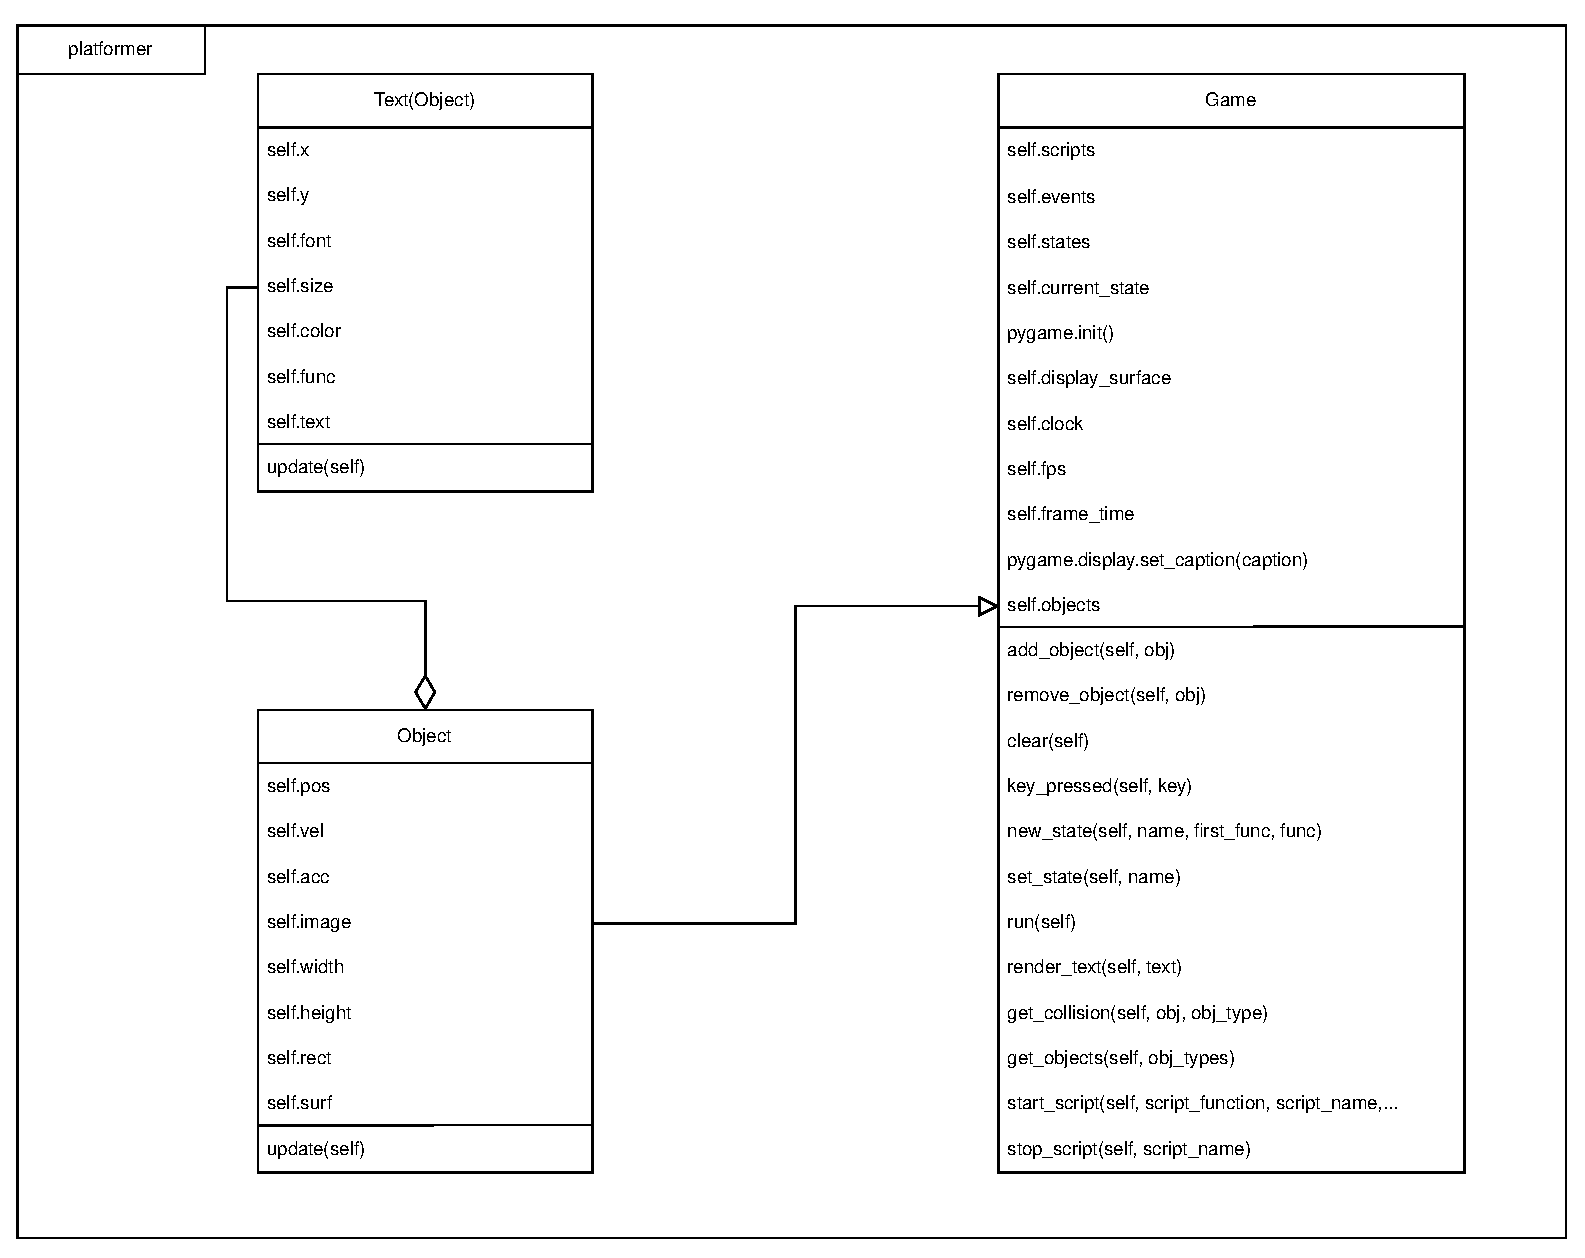
\includegraphics[width=1\linewidth]{platformer}}
	\caption{Диаграмма компонентов platformer}
	\label{platformer:image}
\end{figure}
\paragraph{Описание классов}
\begin{itemize}
		\item[Game] - класс системы платформера. Содержит в себе:
		\begin{enumerate}
				\item self.scripts - словарь для хранения запущенных сценариев;
				\item self.events - cловарь для хранения запущенных event`ов сценариев;
				\item self.states - словарь для хранения состояний игры;
				\item self.current\_state - текущее состояние;
				\item self.display\_surface - создание поверхности дисплея;
				\item self.clock - таймер;
				\item self.fps - количество ФПС(кадров в секунду);
				\item self.frame\_time - длительность кадра;
				\item self.objects.append(obj) - добавление объекта obj в игру;
				\item self.objects.remove(obj) - удаление объекта obj;
				\item self.objects - текущий список объектов;
				\item self.states[name] - создание нового игрового состояния;
				\item self.current\_state - текущее состояние;
				\item self.stop\_script остановка состояния;
				\item self.start\_script - запуск сценария;
				\item self.display\_surface.fill - заливка объекта сплошным цветом;
				\item self.render\_text - обработка текста;
				\item self.display\_surface.blit - отрисовка текстового объекта text;
				\item self.clock.tick - обновление таймера.
		\end{enumerate}
		\item[Object] - класс игрового объекта. Содержит в себе:
		\begin{enumerate}
				\item self.pos - координаты объекта;
				\item self.vel - скорость;
				\item self.acc - ускорение;
				\item self.image - изображение;
				\item self.width - ширина;
				\item self.height - высота;
				\item self.surf - объект для предоставления изображений;
				\item self.rect - прямоугольник;
				\item self.image.get\_width - ширина изображения;
				\item self.image.get\_height - высота изображения.
		\end{enumerate}
		\item[Text] - класс отвечающий за текст. Наследник класса Object. Содержит в себе:
		\begin{enumerate}
				\item self.x - координата x;
				\item self.y - координата y;
				\item self.font - имя шрифта;
				\item self.size - размер шрифта;
				\item self.color - цвет текста;
				\item self.func - функция получения строки текста для реактивного обновления;
				\item self.text - текст.
		\end{enumerate}
\end{itemize}		
Архитектура программы при использования многопоточности также может помочь в достижении более чистой архитектуры проекта. Большинство примеров, которые мы рассмотрим , не обязательно будут работать быстрее используя потоки. Но использование потоков поможет сделать их архитектуру чище и понятнее.
Потоки (Thread)
Стандартная библиотека Python предоставляет библиотеку threading, которая содержит необходимые классы для работы с потоками. Основной класс в этой библиотеки Thread. Чтобы запустить отдельный поток, нужно создать экземпляр потока Thread и затем запустить его с помощью метода .start(). Пример на рисунке \ref{treading:image}:
\begin{figure}[H]
	\begin{lstlisting}[language=Python]
		def start_script(self, script_function, script_name, *args):
			'''
			Запускает сценарий в отдельном потоке с возможностью остановки и передачи аргументов.
			
			:param: script_function: функция, содержащая код сценария
			:param: script_name: имя сценария
			:param: args: дополнительные аргументы, которые передаются в сценарий
			'''
			e = threading.Event()
			self.events[script_name] = e
			
			def func(e, args):
				while not e.is_set():
					script_function(*args)
					time.sleep(self.frame_time)
			
			script_thread = threading.Thread(target=func, args=(e, args))
			script_thread.daemon = True
			script_thread.start()
			self.scripts[script_name] = script_thread
		
		def stop_script(self, script_name):
			'''
			Останавливает сценарий по имени
			
			:param: script_name: имя сценария, который нужно остановить
			'''
			if script_name in self.scripts:
				self.events[script_name].set()
				del self.scripts[script_name]
				del self.events[script_name]
			else:
				# Если сценарий не существует
				print(f"Сценарий {script_name} не существует.")
	\end{lstlisting}  
	\caption{Пример метода tread.start}
	\label{treading:image}
\end{figure}
!!!Когда создается поток Thread, ему передается функцию и список, содержащий аргументы этой функции. В примере указывается Thread, чтобы он запустил функцию thread\_function() и передаем ему 1 в качестве аргумента.

Сама по себе функция thread\_function() мало что делает. Она просто выводит некоторые сообщения с промежутком time.sleep() между ними.
Демоны потоков.
В информатике daemon (демон) – это процесс, который работает в фоновом режиме.

Python потоки имеет особое значение для демонов. Демон потока (или как еще его можно назвать демонический поток) будет остановлен сразу после выхода из программы. Один из способов думать об этих определениях – считать демон потока как потоком, который работает в фоновом режиме, не беспокоясь о его завершении.

Если в программе запущены потоки, которые не являются демонами, то программа будет ожидать завершения этих потоков, прежде чем сможет завершится. Тем не менее, потоки, которые являются демонами, при закрытие программы просто убиваются, в каком бы они состояние ни находились.
join()
Чтобы указать одному потоку дождаться завершения другого потока, вам нужно вызывать .join().  Если вызвать .join(), этот оператор будет ждать, пока не завершится любой вид потока.

Диаграмма состояний ~\ref{State:image}.
\begin{figure}[H]
	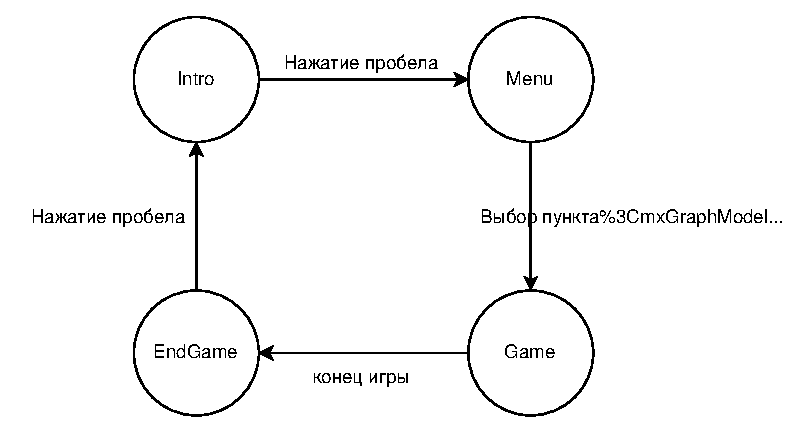
\includegraphics[width=1\linewidth]{State}
	\caption{Диаграмма состояний}
	\label{State:image}
\end{figure}

Диаграмма активности текущего состояния ~\ref{activestate:image}.
\begin{figure}[H]
	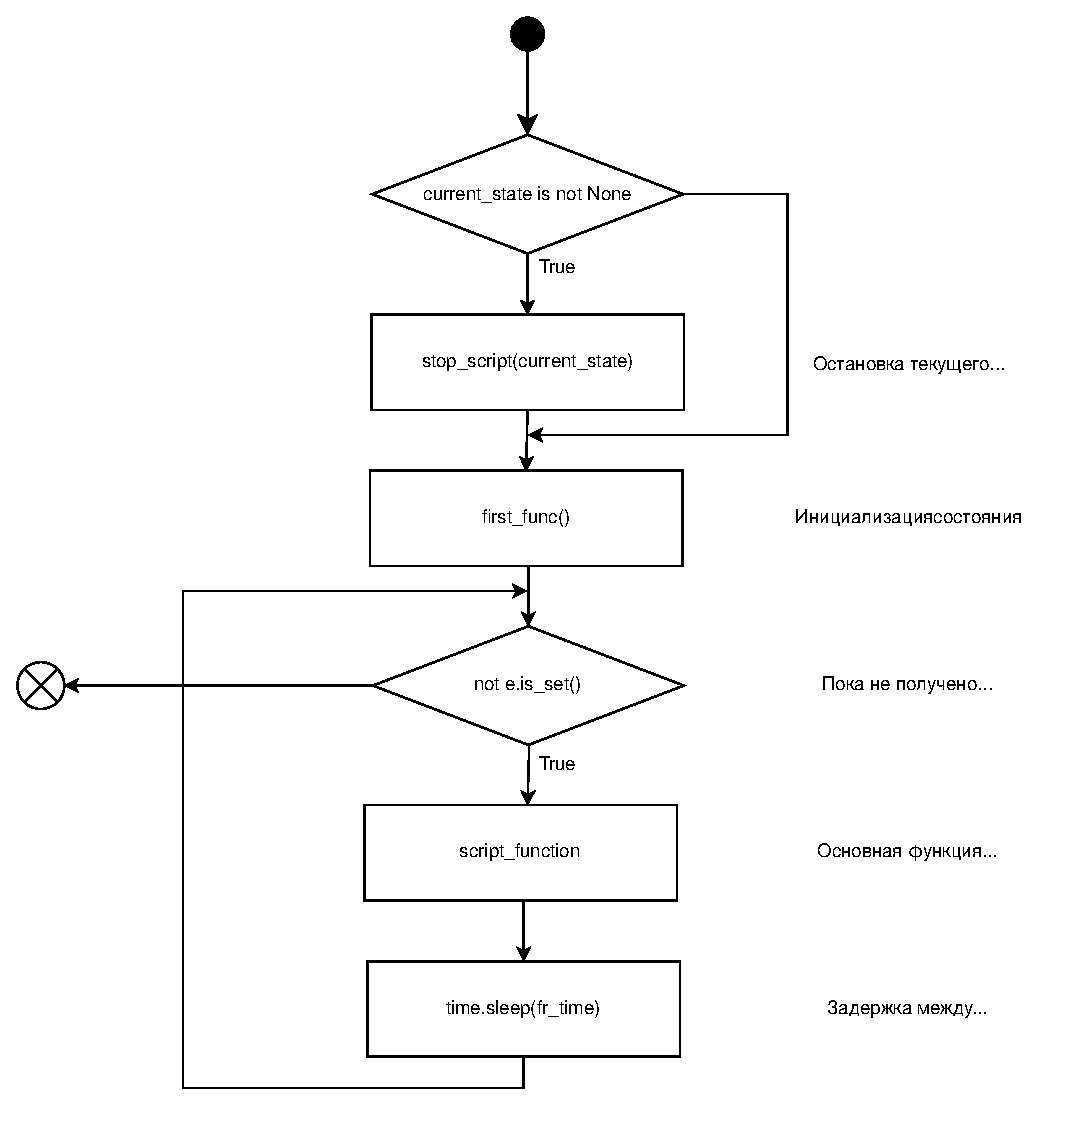
\includegraphics[width=1\linewidth]{activestate}
	\caption{Диаграмма активности текущего состояние}
	\label{activestate:image}
\end{figure}
		
				
\subsection{Пример диаграммы классов игры}

Диаграмма классов игры представлена на рисунке ~\ref{class:image}.
\begin{figure}[H]
	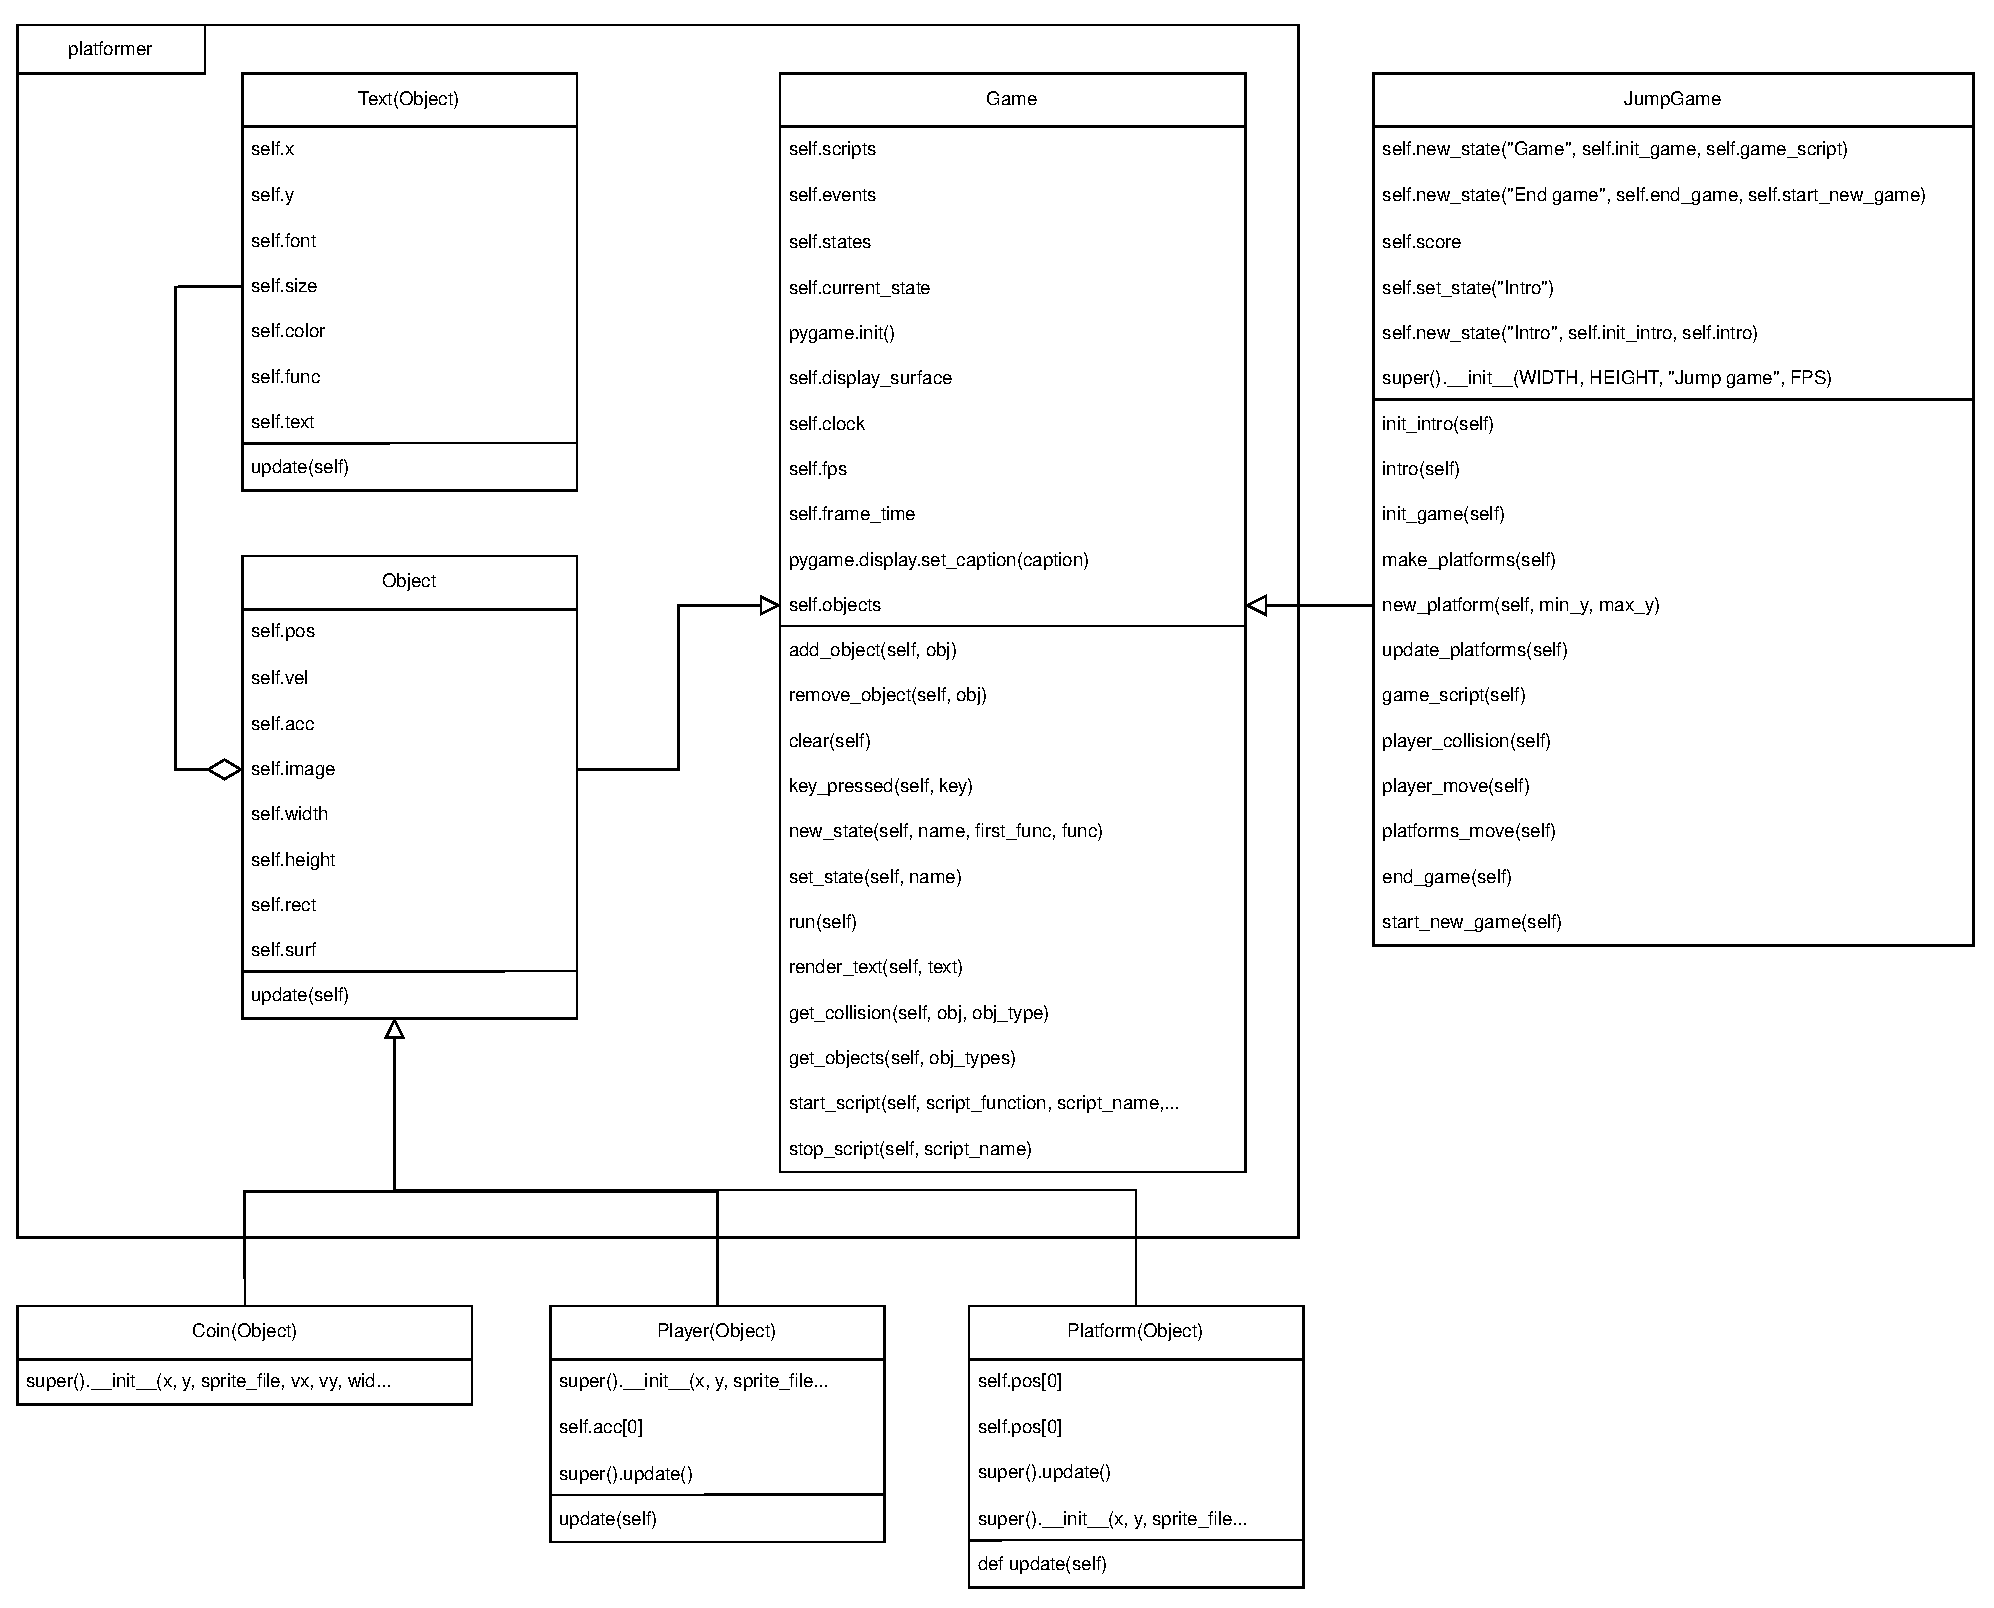
\includegraphics[width=1\linewidth]{class}
	\caption{Диаграмма классов игры}
	\label{class:image}
\end{figure}

 
